\section{Background}\label{sec:background}

% \subsection{Mathematical and numerical background}\label{sec:math-numerical}
\subsection{Conservation Laws}\label{sec:conservation_laws}

Conservation laws form the basis of numerous physical models and are used to describe processes that are stable over time in a given space, e.g., conservation of mass and momentum.
Given below is
the general form of a conservation law for an infinitesimal \gls{2D} fixed Eulerian control volume \autocite{simons2020}:

\begin{equation}\label{eq:general-cl}
	\pdv{\mathbf{q}}{t} + \pdv{\mathbf{f}}{x}  + \pdv{\mathbf{g}}{y} = \mathbf{s}
\end{equation}

It indicates that in the control volume, conserved state variables $\mathbf{q}$ are preserved over time, unless they are changed by fluxes in $x$- or $y$ direction ($\mathbf{f}$ and $\mathbf{g}$ respectively), or a source or sink $\mathbf{s}$, e.g.,  precipitation or infiltration, \autocite{simons2020}.

% \begin{itemize}
% 	\item state variables: $\mathbf{q}$
% 	\item advective and diffusive fluxes in $x$ direction: $\mathbf{f}$
% 	\item advective and diffusive fluxes in $y$ direction: $\mathbf{g}$
% 	\item sources and sinks: $\mathbf{s}$
% \end{itemize}

\subsection{Shallow Water Equations}\label{sec:swe}

The \glspl{swe} are a simplified form of the \gls{rans} equations for shallow surface water flow, for which wavelength is much larger than water depth.
On top of that, we assume
\begin{enumerate*}[label=(\roman*)]
	\item a hydrostatic pressure distribution, and
	\item the negligibility of vertical in comparison to horizontal flow,
\end{enumerate*} 
which enables us to average the \gls{rans} over the water depth, effectively reducing the equations to \gls{2D} space.
% This leads to the population of the variables known from the general form of the conservation law in vector form. \autocite{simons2020}
The variables in the general form of the conservation law (\autoref{eq:general-cl}) are then populated as follows \autocite{simons2020}:

\begin{equation}\label{eq:swe}
	\begin{aligned}
		 & \mathbf{q} = \begin{bmatrix}
			                d  \\
			                ud \\
			                vd
		                \end{bmatrix}, \quad
		\mathbf{f} = \begin{bmatrix}
			             ud                                        \\
			             uud + \frac{1}{2}gd^{2} - \nu \pdv{ud}{x} \\
			             uvd - \nu \pdv{vd}{x}
		             \end{bmatrix}, \quad
		\\
		 & \mathbf{g} = \begin{bmatrix}
			                vd                    \\
			                vud - \nu \pdv{ud}{y} \\
			                vvd + \frac{1}{2}gd^{2} - \nu \pdv{vd}{y}
		                \end{bmatrix}, \quad
		\mathbf{s} = \begin{bmatrix}
			             m_{\mathrm{w}}                                              \\
			             \frac{\tau_{\mathrm{B}x}}{\rho} + gd \pdv{z_{\mathrm{B}}}{x} + f_{x} \\
			             \frac{\tau_{\mathrm{B}y}}{\rho} + gd \pdv{z_{\mathrm{B}}}{y} + f_{y}
		             \end{bmatrix}
	\end{aligned}
\end{equation}

The terms in these vectors are:
\begin{enumerate*}[label=(\roman*)]
	\item the water depth above bottom elevation $d$,
	% \item flow velocity in $x$ direction $u$,
	% \item flow velocity in $y$ direction $v$,
    \item flow velocities $u$ and $v$ in the $x$ and $y$ direction, respectively,
	\item the kinematic viscosity $\nu$, % omitted 
	\item mass sources and sinks $m_{\mathrm{w}}$,
	\item the bed shear stress $\tau_{\mathrm{B}}$,
	\item the bottom elevation $z_{\mathrm{B}}$,
	\item and external forces $f_{x}, f_{y}$. % (omitted) 
\end{enumerate*}

\phantomsection
\label{fix:vector-components}
Mass equilibrium is represented by the first vector components, containing terms for water depth $d$, specific discharges $ud, vd$, and mass sources and sinks $m_w$.
The second and third components describe momentum equilibrium in $x$ and $y$ directions, respectively. 
They include specific discharges $ud, vd$, 
advective fluxes $uud, uvd, vud, vvd$,
viscous fluxes $\nu \pdv{ud}{x}, \nu \pdv{vd}{x}, \nu \pdv{ud}{y}, \nu \pdv{vd}{y}$,
the pressure difference induced momentum transport term $\frac{1}{2}gd^{2}$,
as well as bed friction and bottom slope source terms, $\frac{\tau_B}{\rho}$ and $gd \pdv{z_{B}}{x, y}$, respectively,
and, finally, external forces $f_x, f_y$ \autocite{simons2020}.

% {
% 	\color{Peach}
% 	something about omitted terms?

% 	\begin{equation}\label{eq:swe_canceled}
% 		\begin{aligned}
% 			\rightarrow \; & \mathbf{q} = \begin{bmatrix}
% 																			d  \\
% 																			ud \\
% 																			vd
% 																		\end{bmatrix}, \quad
% 			\mathbf{f} = \begin{bmatrix}
% 										 ud                      \\
% 										 uud + \frac{1}{2}gd^{2} \\
% 										 uvd
% 									 \end{bmatrix}, \quad                 \\
% 										 & \mathbf{g} = \begin{bmatrix}
% 																			vd  \\
% 																			vud \\
% 																			vvd + \frac{1}{2}gd^{2}
% 																		\end{bmatrix}, \quad
% 			\mathbf{s} = \begin{bmatrix}
% 										 m_{w}                                                             \\
% 										 \frac{\tau_{Bx}}{\rho} + gd \pdv{z_{B}}{x} \\
% 										 \frac{\tau_{By}}{\rho} + gd \pdv{z_{B}}{y}
% 									 \end{bmatrix}
% 		\end{aligned}
% 	\end{equation}
% }

% Since the \gls{swe} are given as partial differential equations, they are not solvable analytically in most cases, because the solution gets too complex.
The \glspl{swe} are partial differential equations, to which no general analytical solution is known to exist.
Therefore, numerical solvers are used, which require a discretized version of the \glspl{swe}. 
This is subdivided into spatial discretization, which is described in \autoref{sec:disc-space-FVM}, and temporal discretization, as discussed in \autoref{sec:disc-time}.

% \begin{equation}
% 	\begin{aligned}
% 		 & \mathbf{q} = \begin{bmatrix}
% 			                d  \\
% 			                ud \\
% 			                vd
% 		                \end{bmatrix}, \quad
% 		\mathbf{f} = \begin{bmatrix}
% 			             ud                                                                          \\
% 			             uud + \frac{1}{2}gd^{2} \cancel{ - \nu \pdv{ud}{x} } \\
% 			             uvd \cancel{ - \nu \pdv{vd}{x} }
% 		             \end{bmatrix}, \quad \\
% 		 & \mathbf{g} = \begin{bmatrix}
% 			                vd                                                      \\
% 			                vud \cancel{ - \nu \pdv{ud}{y} } \\
% 			                vvd + \frac{1}{2}gd^{2} \cancel{ - \nu \pdv{vd}{y} }
% 		                \end{bmatrix}, \quad
% 		\mathbf{s} = \begin{bmatrix}
% 			             m_{w}                                                                                \\
% 			             \frac{\tau_{Bx}}{\rho} + gd \pdv{z_{B}}{x} + \cancel{ f_{x} } \\
% 			             \frac{\tau_{By}}{\rho} + gd \pdv{z_{B}}{y} + \cancel{ f_{y} }
% 		             \end{bmatrix}
% 	\end{aligned}
% \end{equation}

\subsection{Discretization of Spatial Derivatives}\label{sec:disc-space-FVM}

There are various approaches for discretizing the spatial derivates of a conservation law, such as \gls{fem}, \gls{fdm}, and \gls{fvm}.
Here, the \gls{ccfvm} is used. This is a form of the \gls{fvm}, which, in contrast to \gls{fdm} and \gls{fem}, is inherently conservative regarding state variables \autocite{hinkelmann2005}.

It discretizes the domain in finitely sized control volumes, also referred to as cells.
The specification \emph{cell-centered} indicates that variables at any point in the cell are computed at the center of the cell and can be reconstructed at other points if needed.
This approach leads to a loss of detail: non-uniform distributions inside the cell are averaged, as the whole cell is treated as a singular unit.
Therefore, a \gls{fvm} model's accuracy is strongly dependent on the cell size
\autocite{simons2020}.

\gls{fvm} is based on the principle of ``integrating the differential equations in their conservative form over all control volumes'' \autocite{hinkelmann2005}.
According to \textcite{simons2020}, utilizing the \gls{fvm}, \autoref{eq:general-cl} is integrated over the domain of the control volume $\Omega$ to:

\begin{equation}\label{eq:int-general-cl}
	\int_\Omega \pdv{\mathbf{q}}{t} \dd{\Omega}
	+ \int_\Omega \left(\pdv{\mathbf{f}}{x} + \pdv{\mathbf{g}}{y}\right) \dd{\Omega}
	= \int_\Omega \mathbf{s} \dd{\Omega}
\end{equation}

Using the Green Gauss Theorem, the flux term can be reduced from a volume integral to a surface integral over the surface of the control volume $\Gamma$, which describes the fluxes through the cell's surfaces \autocite{simons2020}:

\begin{equation}
	\int_\Omega \pdv{\mathbf{q}}{t} \dd{\Omega}
	+ \oint_\Gamma \left(\pdv{\mathbf{f}}{x} + \pdv{\mathbf{g}}{y}\right) \dd{\Gamma}
	= \int_\Omega \mathbf{s} \dd{\Omega}
\end{equation}

These integrals can be solved to gain the spatially discretized form of the conservation law:

\begin{equation}\label{eq:semi-disc-cl}
	\pdv{\mathbf{q}}{t} A
	+ \sum_{k=1}^{n_b} \mathbf{F}_k \mathbf{n}_k l_k
	= \mathbf{s} A
\end{equation}

The reduction from three to two dimensions transforms cell surfaces into edges. 
% Accordingly, \autoref{eq:semi-disc-cl} makes use of
% the flux vector $\mathbf{F}$ and normal vector $\mathbf{n}$, given by $\mathbf{F} \, \mathbf{n} = \mathbf{f}\, n_x + \mathbf{g} n_y$ of the respective edge,
Accordingly, the integral over the cell circumfence can be replaced by the sum over its edges.
In \autoref{eq:semi-disc-cl} the flux vector $\mathbf{F}_k$ represents the flux over an edge. 
It is perpendicular to that respective edge, thus its scalar product with the edge normal vector $\mathbf{n}$ is required, which resolves to $\mathbf{F}_k \, \mathbf{n}_k = \mathbf{f}\, n_x + \mathbf{g} n_y$.
In addition, \autoref{eq:semi-disc-cl} includes
edge index $k$,
length of edge $l_k$,
cell area $A$, and
number of cell edges $n_b$.

\phantomsection
\label{fix:reconstruction}
% To evaluate fluxes $\mathbf{F}$ across a cell's edge, two steps are necessary: the reconstruction of state variables at the edge from their values at the cell center, 
% and the solution of using a flux scheme in the form of a Riemann solver.
% and the actual computation of fluxes from the edge values.
The evaluation of fluxes $\mathbf{F}$ comprises two parts: firstly, the reconstruction scheme and secondly, the flux scheme. The former serves to determine the value of state variables at edges from their stored values at cell centers, and the latter performs the computation of fluxes from edge values.
Some methods, like the \gls{fou} method, combine both 
% requirements, 
parts,
while other flux schemes, like the \gls{hllc} solver introduced in \textcite{toro1994}, require the separate use of a reconstruction scheme.
The first-order reconstruction method uses the values computed at the cell-center at each point in a cell, including at its edge. 
% It is a very simple scheme, but 
While simple, it
causes strong numerical diffusion, leading to a loss in accuracy.
Other reconstruction schemes, like the higher order \gls{tvd} methods, are more accurate, 
but also more complex to implement and computationally intensive.
For details on this, the inclined reader is referred to \textcite{simons2020}.
% As $\mathbf{F}$ describes the flux across a cell's edge and the cell's state is evaluated at its center, reconstruction of these state values is required to calculate $\mathbf{F}$ .
% \note{
% 	einschub zu Flux Schemes, FOU und HLLC droppen
% 	- HLLC braucht vorgeschobenes Rekonstruktionschema, Beispiele fo, TVD
% }

% ``CCFVM-based solvers require the computation of fluxes across cell edges (or faces, in 3D). The SWE solver in hms employs Godunov's method for advective fluxes, using the \gls{hllc} type approximate Riemann solver, as introduced in \textcite{HLLC1994}. This necessitates the reconstruction of cell-based values at the edges, to which end a high-order \gls{tvd} scheme is employed [in \gls{hms}]. Using a \gls{tvd} scheme in the context of Godunov's method forms the so-called \gls{muscl}.'' \autocite{lennart-conf}



% For further details on the \gls{fou} method, as well as the higher order \gls{tvd} methods, the inclined reader is referred to \textcite{simons2020}.

% {
% 	\color{Peach}
	

% 			verschieben in spatial derivatives

% 			Flüsse über Cell edges nötig, first order, überall gleicher wert. Auch komplexere verfahren, zb TVD, siehe Franz oder seine Referenz (wahrschreinlich towards the ultimate conservative diff scheme van Leer) dazu.

% 			doi:10.1016/0021-9991(79)90145-1

	% Computing the flux vector $\mathbf{F}$ has a huge influence on the performance of a \gls{swe} solver, as they include complex calculations \autocite{lennart-hms}.

	% ``CCFVM-based solvers require the computation of fluxes across cell edges (or faces, in 3D). The SWE solver in hms employs Godunov's method for advective fluxes, using the \gls{hllc} type approximate Riemann solver, as introduced in \textcite{HLLC1994}. This necessitates the reconstruction of cell-based values at the edges, to which end a high-order \gls{tvd} scheme is employed [in \gls{hms}]. Using a \gls{tvd} scheme in the context of Godunov's method forms the so-called \gls{muscl}.'' \autocite{lennart-conf}

	% To offer an alternative for the \gls{tvd} scheme, \gls{hms} has recently been extended to implement a first-order reconstruction scheme as well.
% }

\subsection{Discretization of Temporal Derivatives}\label{sec:disc-time}

\autoref{eq:semi-disc-cl} still contains the temporal derivative, which can be discretized using the Forward Euler method. It is equivalent to a first-order Taylor series approximation of the temporal function:

\begin{equation}\label{eq:forward-euler}
	\pdv{\mathbf{q}}{t} \approx \frac{\mathbf{q}^{n+1} - \mathbf{q}^{n}}{\Delta t}
\end{equation}

Applying this to \autoref{eq:semi-disc-cl} results in a fully discretized version of a general conservation law for a finite \gls{2D} cell:

\begin{equation}\label{eq:disc-cl}
	\mathbf{q}^{n+1} =
	\mathbf{q}^n
	- \frac{\Delta t}{A} \sum_{k=1}^{n_b} \mathbf{F}_k^n \mathbf{n}_k l_k
	- \Delta t \, \mathbf{s}^n
\end{equation}
\autoref{eq:disc-cl} describes values at the next %epoch
point in time $t_{n+1}$ based on values of the current %epoch
time $t_n$ only, which makes it an explicit one-step discretization. 
This leads to a low cost per computation at the expense of conditional stability, which is maintained through small time step sizes, as pointed out in the section below.

\subsection{Courant-Friedrichs-Lewy Condition}\label{sec:CFL}

For explicit time stepping to provide a stable solution, it is mandatory to fulfill the \gls{cfl} condition at any point in space and time \autocite{simons2020}.
It is described by the Courant number \Cr, which is required $0 \leq \Cr \leq 1$.
This dimensionless number originates from cell size $\Delta s_i$, maximum propagation velocity $v_{i,\max}$ and time step $\Delta t$ of cell $i$:

\begin{equation}\label{eq:cfl}
	\Cr = \frac{v_{i, \max} \, \Delta t}{\Delta s_i} \leq 1, \quad
	v_{i, \max} = |\mathbf{v}_i| + \sqrt{g d_i}, \quad
	\Delta s_i = \frac{4 \, A_i}{P_i}
\end{equation}

$\Delta s_i$ and $v_{i,\max}$ consist of the components
absolute flow velocity $|\mathbf{v}_i|$,
gravity constant $g$,
water depth $d_i$,
cell area $A_i$, and
cell perimeter $P_i$

Many explicitly discretized applications use a preset Courant number $\Cr \in [0.3, 0.8]$ to set the time step $\Delta t$ 
% \autocite{sanders2008,simons2020,steffen2023,hu2019,dazzi2018}.
\autocite{dazzi2018,hu2019,sanders2008,simons2020,steffen2023}.
Thus, $\Delta t$ is adapted to the current need, reducing computational effort when facing slower flow velocities on a static domain of cells.

\begin{equation}\label{eq:cfl-time-step}
	\Delta t = \min \left( \frac{\Cr \, \Delta s_i}{v_{i, \max}} \right)
\end{equation}

% \note{
% 	or rather put i in range somewhere
% 	$$ \Delta t = \min_{i=0}^{n_c} \left( \frac{\Cr \, \Delta s_i}{v_{i, \max}} \right) $$
% }

To fulfill the \gls{cfl} condition, the smallest time step of all $n_c$ cells is applied as the time step for the whole domain.
Consequently, high velocities in a small portion of the domain impact the whole domain's next time step, which increases the model's overall runtime linearly.
This approach forms a scheme called \gls{gts}, the basic time stepping scheme for \gls{fvm} solvers.

\subsection{Local Time Stepping}\label{sec:LTS}

While \gls{gts} has proven reliable in many applications involving \gls{fvm} models, ``model efficiency suffers using non-uniform grids and uniform grids with variable 
% $a$ 
[maximum propagation velocity] 
because the Courant number in many cells is far 
% less than one% original citation
[below its limit]% we already introduced a range of [0.3, 0.8], whose lower limit i'd already consider "far less than one".
'' \autocite{sanders2008}.
The author refers to non-uniform grids as ones with varying cell sizes, e.g., varying cell length in a \gls{1D} scenario, distortions in a structured \gls{2D} grid or an unstructured \gls{2D} grid. 

\begin{figure}[htbp]
	\centering
	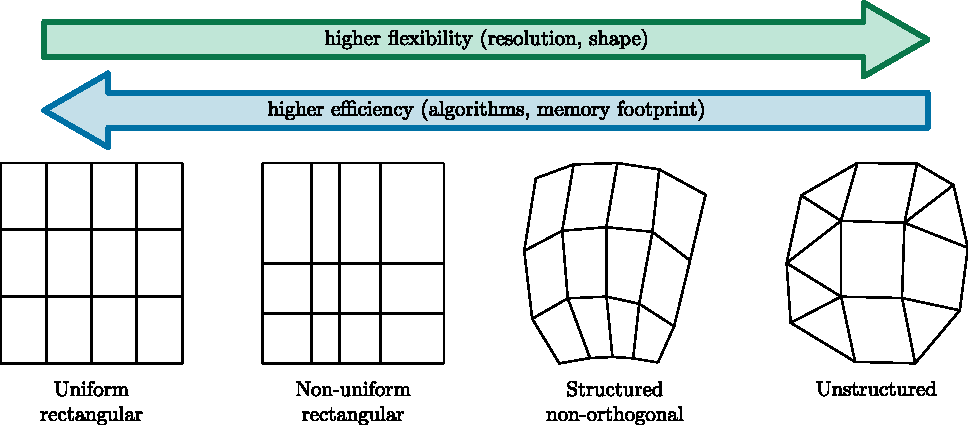
\includegraphics[width=\textwidth]{./img/grid_types.pdf}
	\caption{Typology of \acrshort{2D} grids \autocite{lennart-hms}}
\end{figure}

To improve efficiency, \textcite{osher1983} have developed the concept of \gls{lts}. They proved that a local \gls{cfl} condition is sufficient to provide a correct solution for nonlinear conservation laws in \gls{1D} domains.
Therefore, given a constant Courant number $\Cr$,
the time step can be adapted to each cell $i$
in conformity with maximum propagation velocity $v_{i, \max}$ and cell size $\Delta s_i$:
\begin{equation}\label{eq:local-time-step}
	\Delta t_i = \frac{\Cr \, \Delta s_i}{v_{i, \max}}
\end{equation}
For uniform grids, i.e., fixed-size cells, $\Delta s_i$ is constant across the whole domain, leaving  $v_{i, \max}$ as the only factor impacting the local time step $\Delta t_i$.

\textcite{crossley1999} were the first to apply \gls{lts} in the field of computational hydraulics. They used the Saint-Venant Equations, a \gls{1D} version of the \glspl{swe}, to model open channel flow and tested two \gls{lts} methods on it.
In a later publication, that included examinations on non-uniform grids among others, they found that the performance gain provided through \gls{lts} increases with the ratio of the largest to the smallest cell lengths \autocite{crossley2003}.
They also pointed out that interactions of adjacent cells require attention to guarantee a correct exchange of information about their current state \autocite{crossley2003}.
In particular, they compared two approaches to \gls{lts}: \emph{\gls{frozen-flux-LTS}} by \textcite{zhang1994a} and \emph{Full Time Integration} by \textcite{kleb1992}.
The latter of which can be categorized as a \gls{pow2-LTS} and was found to be more effective at reducing runtime on both uniform and non-uniform grids.
Both methods were initially developed for the field of aeronautics and astronautics.

\subsubsection{Frozen Flux LTS}
\Acrfull{frozen-flux-LTS} focuses on optimizing flux calculations. Because of their complexity, they account for a large part of a model's runtime.
\phantomsection\label{fix:tvd-fo-cost}This complexity varies, depending on the chosen reconstruction scheme. 
When using higher order schemes, like \gls{tvd} methods, reconstruction can be held accountable for a significant fraction of computational cost.
% \note{maybe move this to other part about reconstruction}
% This is substantially due to the costly reconstruction of edge values from the cell center. 
% naja. Auch bei first order hat die Flussberechnung den größten Anteil. Das müsstest du umformulieren, z.B. so, dass high-order reconstruction schemes dies noch verstärken können.

\textcite{zhang1994a} introduced an \gls{lts} method based on reducing the total amount of flux updates.
They achieved this by \emph{freezing} fluxes and reusing them as long as permitted by their local \gls{cfl} condition.
The following procedure is an adapted version of this scheme. The original authors used a different nomenclature and illustrated it using the \gls{1D} unsteady Euler equations instead of the \glspl{swe}.

Assuming a constant global time step $\Delta t$, we can infer that fluxes of cell $i$ can be reused $j_{\max}$ times, given by:

\begin{equation}\label{eq:reuse-number}
	% j_{\max} \, \Delta t \leq
	% \Delta t_i \leq
	% (j_{\max} + 1)	 \, \Delta t
	% \quad \rightarrow \quad
	j_{\max} = \left\lfloor \frac{\Delta t}{\Delta t_i} \right\rfloor
\end{equation}

Using this on \autoref{eq:disc-cl}, we can deduce the state at all intermediary global time steps $\mathbf{q}^{n+j}, \, j \in [1,j_{\max}]$.
To enhance readability, we substitute the flux term with a helper variable $\boldsymbol\Phi^n = \sum_{k=1}^{n_b} \mathbf{F}_k^n \mathbf{n}_k l_k$.

\begin{equation}\label{eq:frozen-flux-LTS}
	\begin{aligned}
		\mathbf{q}^{n+j}
		= \mathbf{q}^n
		- \frac{j\, \Delta t}{A_i} \boldsymbol\Phi^n
		- \sum_{j=1}^{j_{\max}}
		\Delta t \, \mathbf{s}^{n+j-1}
	\end{aligned}
\end{equation}

While the fluxes remain unchanged, state variables are updated each global time step $\Delta t$, so exchanging information at cell interfaces is possible at all times.

A more thorough explanation of the scheme can be found in \textcite{zhang1994a}.

Compared to a \gls{gts}, the \gls{frozen-flux-LTS} reduced the number of flux updates by approximately 67\% in multiple test cases, deducted by \textcite{crossley2003}.
Additionally, both \textcite{crossley2003, zhang1994a} found that accuracy can improve through the use of this scheme when comparing results with analytical solutions.
This effect is explained by the reduction of local truncation error \autocite{crossley2003,zhang1994a}

\subsubsection{Power-of-two Level based LTS}

An alternative approach to \gls{lts} consists of skipping a set of time steps at parts of the domain altogether: the \acrfull{pow2-LTS} scheme.
The idea is to cluster cells in proportion to their local time steps $\Delta t_i$ into groups that share an \gls{lts}-level $m_i$, which determines a shared local time step used for these cells: $\Delta t_m$.

\begin{equation}\label{eq:pow2-lts-level}
	m_i = \left\lfloor
	\log_2 \frac{\Delta t_i}{\Delta t_{\mathrm{base}}}
	\right\rfloor
\end{equation}

These level time steps are defined by an exponential function that scales the base time step: $\Delta t_m = 2^m \Delta t_{\mathrm{base}}$. 
Many implementations use the global minimum time step as their base \autocite{kleb1992,crossley2003,dazzi2018,yang2020}; others utilize a predefined constant instead \autocite{sanders2008}.

As such, all cells regularly synchronize to exchange information, as depicted in \autoref{fig:pow2-LTS}.
At interfaces of different \gls{lts}-levels, intermediate values of the larger level are interpolated on demand.
To maintain a stable solution, it is suggested to introduce intermediate regions between directly adjacent cells, which differ by more than one level \autocite{crossley2003}, forming a method called level smoothing and is discussed later on in \autoref{sec:LTS-smoothing}.

The \gls{pow2-LTS} consists of performing a sequence of level loops, reaching from time $t_n$ to $t_n + \Delta t_{\max}$, where $\Delta t_{\max}$ is the time step of the largest level. 
In a level loop, the largest level is advanced by a single time step. 
All other levels are advanced until they synchronize again, i.e., all cells are advanced to $t_n + \Delta t_{\max}$.
The base time step $t_{\mathrm{base}}$ is required to stay constant within a level loop.

At the start of a level loop, each cell is assigned a level (\autoref{eq:pow2-lts-level}).
Then, each cell is updated once. As their local time steps vary, they are updated to different points in time $t_n$.
Following this, the lower levels are updated in a way that they catch up with the highest level, so that finally, all regions are synchronized, and level assignment can be re-evaluated for the next loop.
Further details of the scheme can be found in \textcite{kleb1992,crossley2003}.

\begin{figure}[htbp]
	\centering
	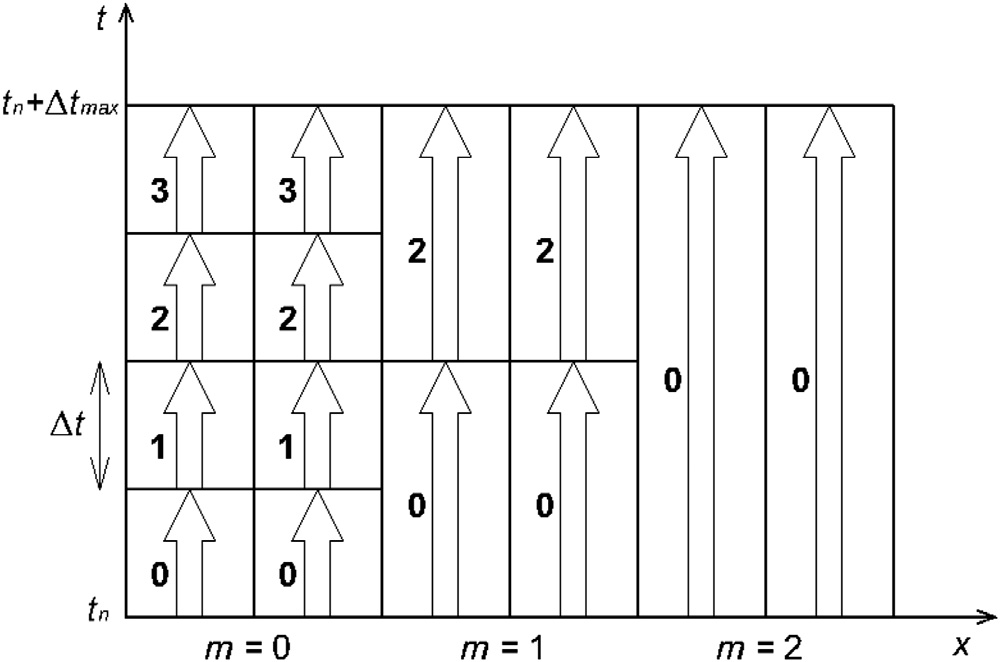
\includegraphics[width=0.6\textwidth]{img/dazzi2018_fig3.jpg}
	\caption[\Acrlong{pow2-LTS} scheme]{
		\Acrlong{pow2-LTS} scheme with three levels showing a level loop, i.e., a full synchronization cycle \autocite{dazzi2018}.
	}
	\label{fig:pow2-LTS}
\end{figure}

Compared to a \gls{gts}, the \gls{pow2-LTS} reduced the number of flux updates by 61\%-66\% in multiple test cases deducted by \textcite{crossley2003}.
While \gls{pow2-LTS} is exceeded by \gls{frozen-flux-LTS} in this metric, it still outperforms the other scheme in terms of runtime: it achieves a mean reduction of 50.8\% in contrast to 27.3\% for \gls{frozen-flux-LTS}, according to the authors.
They state this is due to the need of the latter to update state variables each local time step \autocite{crossley2003}.

\subsubsection{2D LTS}

\textcite{sanders2008} has further evolved \gls{lts} in the domain of hydraulics simulations by proposing a scheme applicable to \gls{2D} models.
Similarly to \textcite{crossley2003}, the author points out, that models using uniform grids might benefit from \gls{lts}, if they have a large spatial heterogeneity in maximum propagation velocity.

His scheme adopts first-order reconstruction and a \gls{pow2-LTS} method with a predefined base time step, which is constant throughout the simulation \autocite{sanders2008}.
While proving useful in general, he reported stability problems on wet/dry fronts, especially when using more than four \gls{lts}-levels, which led him to the conclusion that it should be limited to four in practical applications. 
He was able to reduce runtime by 50--70\% without loss of accuracy for applications of four levels.
As an aside, his approach generally showed better performance and stability when bed friction was included in the models.

These stability problems were successfully targeted by \textcite{hu2019}, who introduced changes to the calculation of the allowable local time step for almost-dry cells and interface regions, which smoothen borders between different levels.

\subsubsection{Interfaces of Divergent Regions}\label{sec:LTS-smoothing}

As mentioned above, many \gls{lts} schemes utilize techniques to even out interfaces between regions whose time steps diverge \autocite{crossley2003,sanders2008,dazzi2018,hu2019,yang2020}.
The main purpose is to limit instabilities and improve accuracy, as waves can be propagated from a cell with a small time step to an adjacent one with a larger time step within a single level loop in a \gls{pow2-LTS} scheme \autocite{crossley2003}.

There are two popular approaches: (a) neighbor propagation and (b) introducing interface regions.

The former compares a cell with all adjacent cells (neighbors) and chooses the minimum of their local time steps as the cell's allowable time step $\Delta t_i$ \autocite{sanders2008,yang2020}.
In the case of \gls{pow2-LTS}, 
% it is still possible to have neighbors with more than one level difference, 
% neighboring levels may still differ by more than one, 
%oder vllt
adjacent cells may still differ by more than one level,
since only direct neighbors are taken into account.

The latter establishes a region in which the local time step $\Delta t_m$ is gradually increased to provide a smooth transition. 
% However, the specifics of these approaches are beyond the scope of this thesis and can be viewed in other publications 
For further details on these approaches, the inclined reader may refer to the respective publications
\autocite{crossley2003,dazzi2018,hu2019,kleb1992}.

\subsection{Scope and Purpose of \texorpdfstring{\hms}{hms++}}\label{sec:hms-scope-purpose}

The \gls{hms} is an open-source numerical solver for the \glspl{swe} written in C++ with performance and user-friendliness in mind. 
It is developed at TU Berlin's Chair of Water Resources Management and Modeling of Hydrosystems and forms the successor to the Hydroinformatics Modeling System (hms) Java framework.

At its core are \gls{ccfvm} spatial and explicit Euler temporal integration in combination with a first-order and a \gls{tvd} scheme for flux reconstruction.
\gls{hms} can handle unstructured and multiple variations of structured meshes.
Details are provided in \textcite{lennart-conf,lennart-hms}.

% A core motivation of the development of \gls{hms} was to enable the use of \gls{2D} \gls{swe} models in large-scale systems by shifting 
% % the upper applicability limit of the latter.
% their applicability limit.
% The lower limit consists of considerations whether a model can represent a certain detail relevant for a specific task, and can be thought of as a \emph{hard limit}.
% In contrast, the upper limit can be regarded simply as the cost and practicability of running a simulation and therefore a \emph{soft limit}
% \autocite{lennart-hms}.

% \begin{figure}[htbp]
% 	\centering
% 	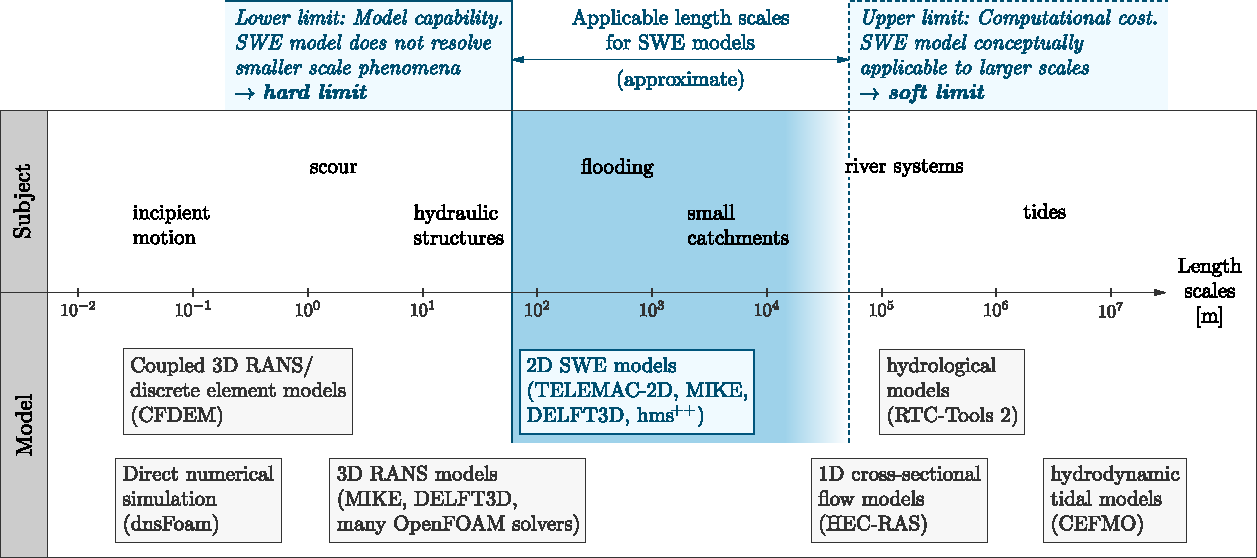
\includegraphics[width=\textwidth]{./img/length_scales_rev.pdf}
% 	\caption
%     [Subjects of interest in fluid flow at their characteristic length scales]
%     {
% 		``Subjects of interest in fluid flow at their characteristic length scales, and models (with software examples in brackets) at their applicable length scales (approximate).''
% 		\autocite{lennart-hms}
% 	}
% \end{figure}

\gls{hms} aims to shift the \glspl{swe}' applicability limit, to enable their use in larger cases, currently restricted by the cost of computation, see \autoref{sec:intro}.
To achieve this, both \gls{simd} and \gls{mimd} parallel processing, as well as methods for optimally utilizing CPU cache are employed. 
\gls{simd} parallelism is provided through the use of the \emph{Eigen} library for linear algebra, which features clean and easily readable source code while optimizing matrix and vector operations in the background by adapting to specific CPU capabilities.
\gls{mimd} parallelism is implemented using \gls{omp} for coordinating threads on a single node and \gls{mpi} for communication between multiple compute nodes.
Each thread is supplied with pre-allocated buffers, which are reused throughout the runtime
\autocite{lennart-hms}.

% \note{I don't think I'm going need plugin/coupling + usability here}

% \paragraph*{Blockwise Partitioning in \texorpdfstring{\hms}{hms++}}\label{sec:hms-block}
When computing simulations with uniform rectangular meshes, \gls{hms} can group cells into blocks to facilitate \gls{simd}.
It is able to carry out operations efficiently on multiple cells at once through vectorized functions implemented in \emph{Eigen}.
Additionally, \gls{mimd} is used to distribute blocks across multiple threads or compute nodes.
Such block-wise traversal has shown performance gains of 14--25 times in comparison to classic cell-wise traversal of the domain \autocite{lennart-hms}.
